\section{Setting up the Workspace for Java Projects}

After installation of eclipse and the \eTrice{} plug in, your workspace should look like this:  

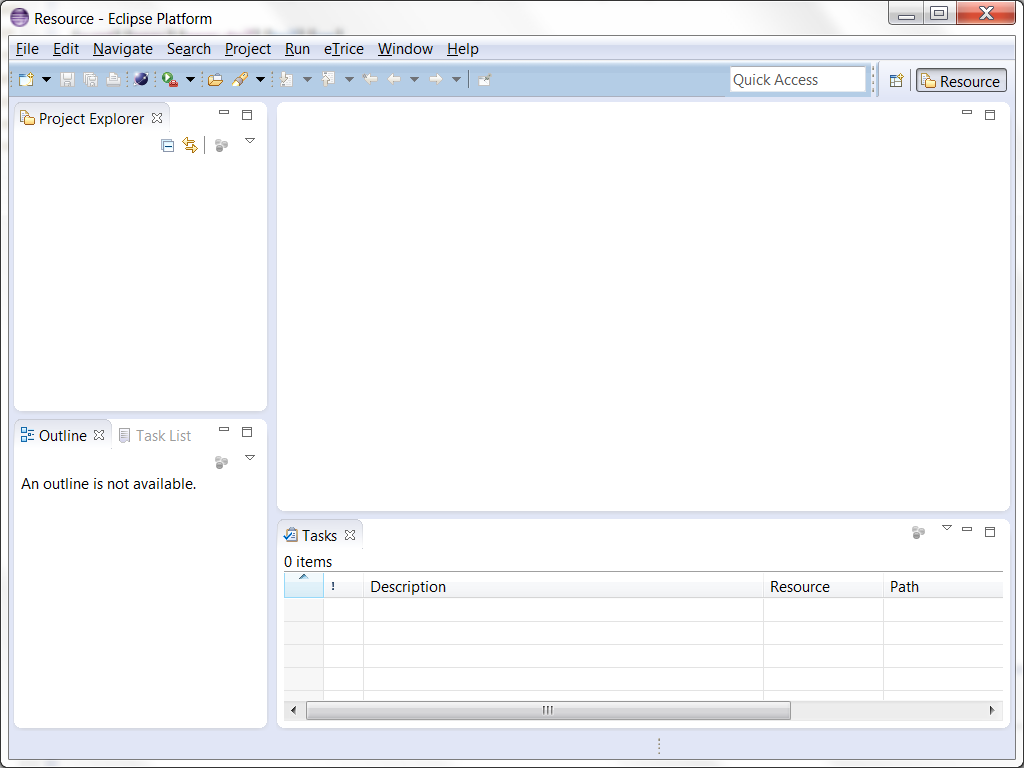
\includegraphics[width=0.8\textwidth]{images/013-SetupWorkspace01.png}
% !images/013-SetupWorkspace01.png!

Just the \textit{\eTrice{}} menu item is visible of the installed \eTrice{} plugins.

Select the menu \emph{File->New->Other}

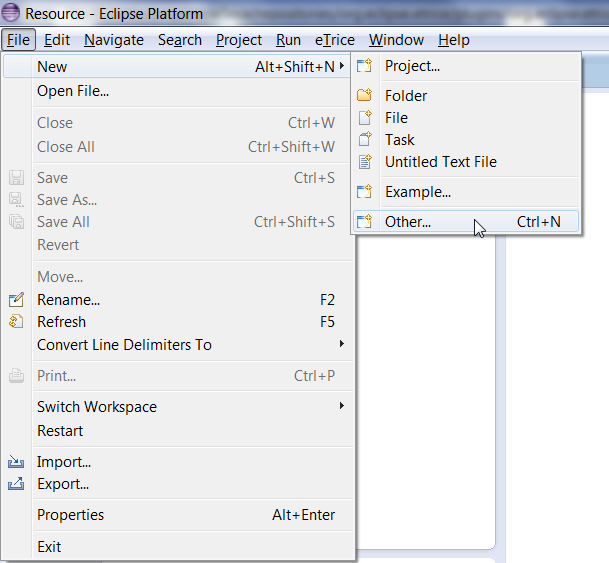
\includegraphics[width=0.8\textwidth]{images/013-SetupWorkspace02.png}
% !images/013-SetupWorkspace02.png!

Open the \textit{\eTrice{}} tab and select \textit{\eTrice{} Java Runtime}

Press \textit{Next} and \textit{Finish} to install the Runtime into your workspace.

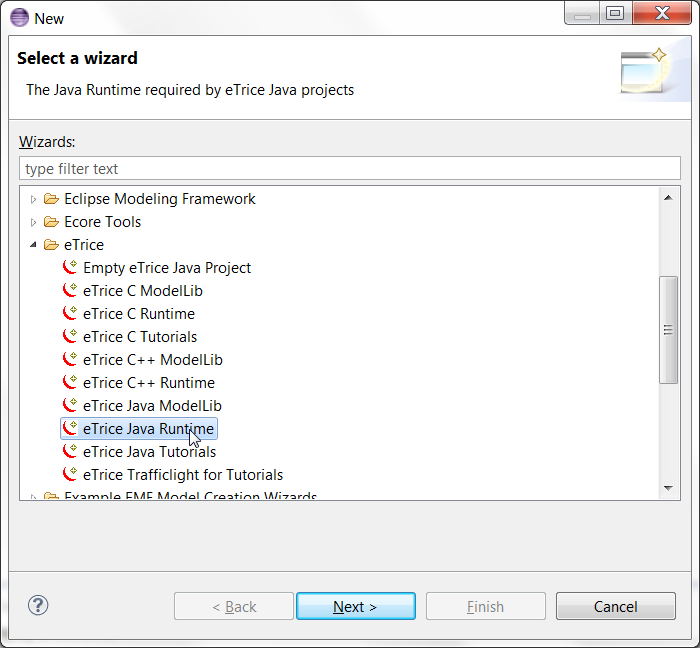
\includegraphics[width=0.8\textwidth]{images/013-SetupWorkspace03.png}
% !images/013-SetupWorkspace03.png!

Do the same steps for \textit{\eTrice{} Java Modellib} and \textit{\eTrice{} Java Tutorials}. To avoid temporary 
error markers you should keep the proposed order of installation. The resulting workspace should look like 
this:

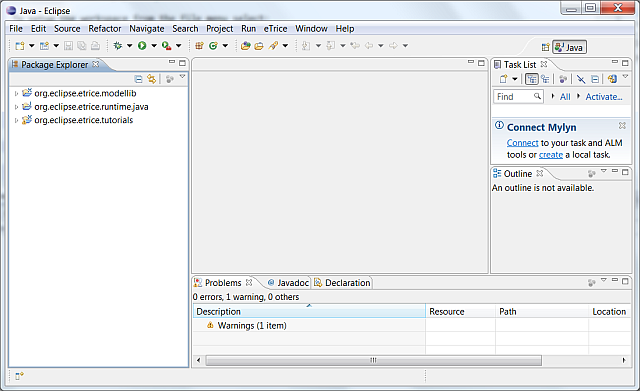
\includegraphics[width=0.8\textwidth]{images/013-SetupWorkspace04.png}
% !images/013-SetupWorkspace04.png!

Now workspace is set up and you can perform the tutorials or start with your work.

The tutorial models are available in the \textit{org.eclipse.etrice.tutorials.java} project. All tutorials are 
ready to generate and run without any changes. To start the code generator simply run 
\emph{gen\_org.eclipse.etrice.tutorials.java.launch} as \emph{gen\_org.eclipse.etrice.tutorials.java}: 

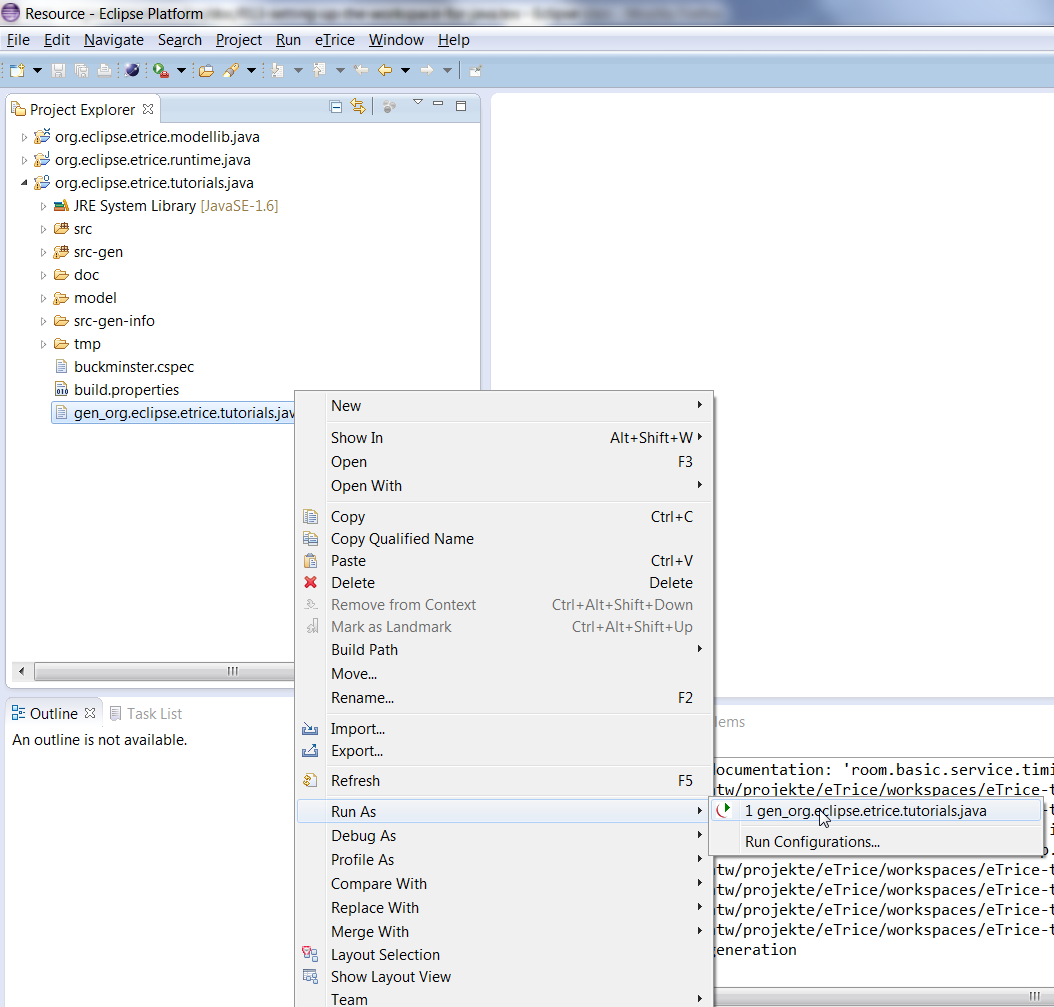
\includegraphics[width=0.8\textwidth]{images/013-SetupWorkspace05.png}
% !images/013-SetupWorkspace05.png!

The successful generation ends with \emph{Info: -- finished code generation} in the Console.

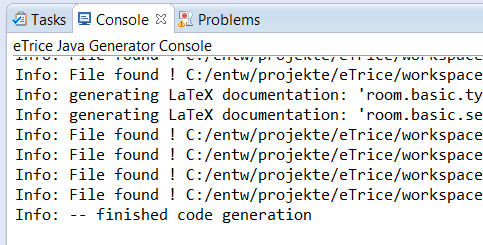
\includegraphics[width=0.8\textwidth]{images/013-SetupWorkspace051.png}
% !images/013-SetupWorkspace051.png!


For each tutorial in the folder src-gen a java package is generated including a java file called 
\emph{SubSystem\_<Modelname>Runner.java} . To run the a generated application simply run this file as a java application.
Try this with the file \emph{src-gen/HelloWorld/SubSystem_HelloWorldRunner.java} :

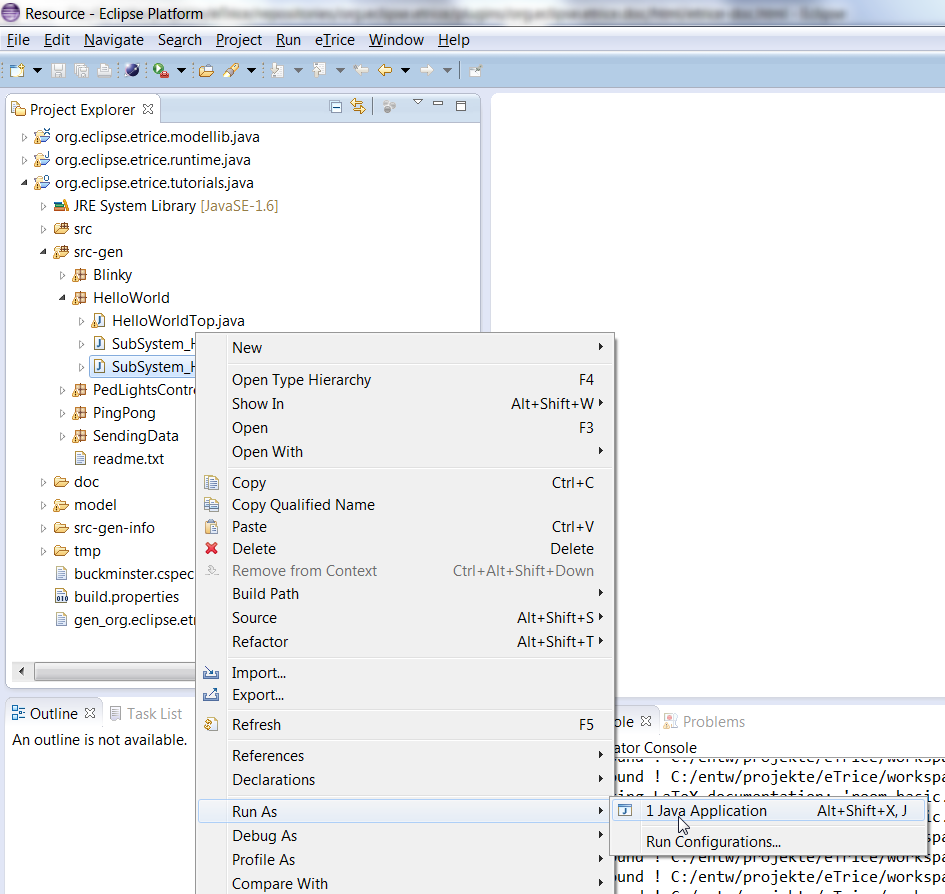
\includegraphics[width=0.8\textwidth]{images/013-SetupWorkspace06.png}
% !images/013-SetupWorkspace06.png!

To stop the application type \emph{quit} in the console window.
 
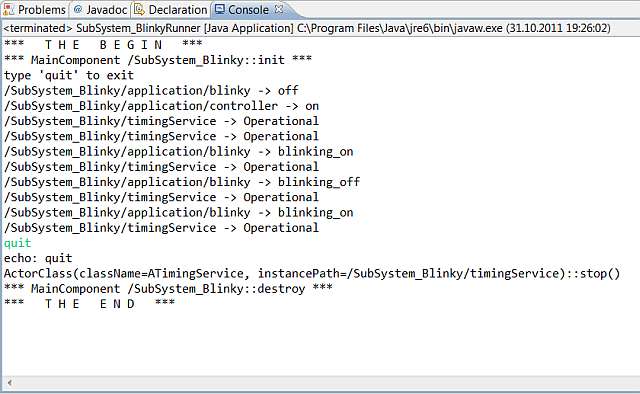
\includegraphics[width=0.8\textwidth]{images/013-SetupWorkspace07.png} 
% !images/013-SetupWorkspace07.png!

Performing the tutorials will setup a dedicated project for each tutorial. Therefore there are some 
slight changes especially whenever a path must be set (e.g. to the model library) within your own 
projects. All this is described in the tutorials.
